\documentclass[hyperref, lof, lot, noproblem, masterofscience]{cgvpub}
\graphicspath{{./images/}}
\usepackage{multirow}
%weitere Optionen zum Erg�?nzen (in eckigen Klammern):
%
% bibnum	numerische Literaturschl�?ssel
% final 	f�?r Abgabe
% lof			Abbildungsverzeichis
% lot			Tabellenverzeichnis
% noproblem	keine Aufgabenstellung
% notoc			kein Inhaltsverzeichnis
% twoside		zweiseitig
\author{Xiaoyu Yin}
\title{Translating Natural Language to SPARQL}
\birthday{13. June 1994}
\placeofbirth{Zhumadian}
\matno{4572954}
\betreuer{Dr. Dagmar Gromann}
\bibfiles{literature}
\problem{Text der Aufgabenstellung...}
\copyrighterklaerung{Copyright information here}
\acknowledgments{Acknowledgments here blablabla}
\abstracten{English abstract here}
\abstractde{Zusammenfassung Text Deutsch?}
\begin{document}


\chapter{Introduction} \label{chapter:introduction}


% Chapter Introduction

% What would be included in this chapter?
This chapter provides an introduction of the thesis. We introduce the motivation of this thesis in section \ref{section:motivation}, and the outline of this thesis in section \ref{section:thesis outline}.

% Section Motivation

\section{Motivation} \label{section:motivation}
% Short description of what is Linked Data, Question Answering, SPARQL. What is the relationship between these concepts? What is the current situation and what are the current demands? What is the (goal) task of this thesis? Why is it important to realize this goal? why is it useful to translate natural language to SPARQL? Who can benefit from it and how can they benefit from it?
In recent years, numerous documents have been published onto the web in a fast-growing speed, forming a global information space which worldwide people have access to. 

\section{Thesis Outline} \label{section:thesis outline}
% How many chapters does this thesis have? What are the main contents that would be described in each chapter? 

Chapter \ref{chapter:background} presents the background of this thesis.

Chapter \ref{chapter:methodology} describes the research method used in this thesis.

Chapter \ref{chapter:experiments} shows the experiments conducted during this thesis.

Chapter \ref{chapter:analysis} depicts the analysis derived from the experiment results.

Chapter \ref{chapter:conclusion} concludes the whole thesis and provides potential directions for the future work.


\chapter{Background} \label{chapter:background}


% Chapter Background
This chapter introduces the background knowledge involved in this thesis. Semantic Web Technologies is briefly introduced in section \ref{section:semantic web technologies}, including the notion of Linked Data in section \ref{subsection:linked data} and SPARQL in section \ref{subsection:sparql}. Section \ref{section:neural machine translation} introduces the field of neural machine translation. Related research is discussed in section \ref{section:related work}.

\section{Semantic Web Technologies} \label{section:semantic web technologies}

The World Wide Web has changed the livings of people dramatically. It enables people from all over the world to browse, share, and communicate large amount of information in an unprecedented speed. This communication is based on the exchange of distributively stored documents of different kinds and formats. For a client-side user, the most common way of establishing such communication is by entering keywords, phrases, or sentences into a chosen search engine, and retrieving desired information from the result list of websites. 

\subsection{Linked Data} \label{subsection:linked data}
% What is Linked Data? What is the use of Linked Data? 

\subsection{SPARQL} \label{subsection:sparql}
% What is SPARQL


\section{Neural Machine Translation} \label{section:neural machine translation}

\subsection{Sequence to Sequence Learning}


\subsection{Recurrent Neural Network}


\subsection{Long Short-Term Memory}


\section{Related Work} \label{section:related work}

The primary focus of the investigation in this thesis is the neural network models that can be used to map natural language statements to SPARQL expressions. Despite that such models usually just perform the role of sequence to sequence learning, the specialty of SPARQL as a structured language with strictly defined syntax and vocabulary often lead to highly different experiment results compared to the common machine translation tasks where the source and target sequence are both unstructured. Therefore, we only consider all the research which deployed machine learning methods to map unstructured sequences to structured sequences as the most related work.

\cite{Cai2017} proposed an enhanced encoder-decoder framework for the task of translating natural language to SQL, a similar query language with SPARQL but targeting structured databases instead of knowledge bases. They used not only bleu, but also query accuracy, tuple recall, and tuple precision for measuring the quality of output queries, and achieved good results.

\cite{Soru2018a,Soru2018} proposed a generator-learner-interpreter architecture, namely Neural SPARQL Machines to translate any natural language expression to encoded forms of SPARQL queries. They designed templates with variables that can be filled with instances from certain kinds of concepts in target knowledge base and generated pairs of natural language expression and SPARQL query accordingly. After encoding operators, brackets, and URIs contained in original SPARQL queries, the pairs were fed into a sequence2sequence learner model as the training data. The model was able to predict on unseen natural language sentence, and generate encoding sequence of SPARQL for interpreter to decode. 



\chapter{Methodology} \label{chapter:methodology}


This chapter mainly describes the models of neural machine translation involved in this thesis for the task of translating natural language to SPARQL and related preliminaries. Then, a measurement BLEU that is typically utilized in automatic machine translation evaluation is described. We also clarify another metric called query accuracy which suits for our task specifically.

\section{Preliminary}

\subsection{SPARQL Encoding} \label{subsection:preprocessing}

Unlike natural language, SPARQL queries are often written in structured forms instead of sequences that are easy to be tokenized. Therefore, the first step of training a Seq2Seq model with SPARQL is to convert SPARQL queries into sequences. To clarify, we encode the original SPARQL query into a sequential form which can be later decoded back. 

We adopted the encoding approach in \cite{Soru2018a}, which basically applies the following operations:
\begin{enumerate}
\item shorten the entities in the query with prefixes
\item replace the built-in symbols with dedicated words connected with underscores
\item shorten the query by replacing the built-in set phrases (e.g. \texttt{ORDER BY}) with one simplified word
\end{enumerate}

These operations can be implemented as a set of replacements and applying them turns an original SPARQL query to a final sequence which contains tokens that are only formed of characters and underscores. An example is shown in Table \ref{table:sparql encoding}. After training, as an encoded form of SPARQL translation is generated, it can be easily decoded back by reverse replacements.

\begin{table}[h]
\begin{tabular}{c | p{0.9\textwidth}}
SPARQL & \begin{lstlisting}[language=SPARQL]
SELECT DISTINCT ?uri 
WHERE { 
<http://dbpedia.org/resource/Sam_Loyd> <http://dbpedia.org/ontology/knownFor> ?uri .
<http://dbpedia.org/resource/Eric_Schiller> <http://dbpedia.org/ontology/knownFor> ?uri . 
}
\end{lstlisting} \\
\hline
Encoded & {\small select distinct var\_uri where brack\_open dbr\_Sam\_Loyd dbo\_knownFor var\_uri sep\_dot dbr\_Eric\_Schiller dbo\_knownFor var\_uri sep\_dot brack\_close}
\end{tabular}
\caption{A SPARQL query is encoded into a sequence of short tokens before treated as the input of the seq2seq model. Thus, the model learns how to translate from natural language texts into sequences of encoded form of SPARQL.}
\label{table:sparql encoding}
\end{table}



\subsection{Input} \label{subsection:preliminary input}

For the input of the NMT models, a sentence or paragraph can be normally separated into three kinds of sequences: characters, subwords, or words. Different methods of splitting sequences lead to differences in vocabularies that are seen by the model and its effectiveness of dealing with rare words. For the task in this thesis, the texts are fed into the models in a word-based fashion on account of the reason that the words contained in the SPARQL vocabulary are mostly SPARQL operators and DBpedia entities that need to be treated as a whole.

\begin{figure}[h]
\includegraphics[width=0.5\textwidth]{one-hot_encoding}
\centering
\caption{For our task, the source input (left) and target input (right) are one-hot encoding vectors representing word positions from respectively English and SPARQL vocabulary. The output vector is a probability distribution over all words in SPARQL vocabulary.}
\label{figure:one-hot encoding}
\end{figure}

Each word in the sequences of both source input and target input is represented as an one-hot encoding vector, which is a sparse vector in which one element is set to 1 and all other elements are set to 0. The dimension of the one-hot encoding is equal to the size of the specific vocabulary. An example is shown in Figure \ref{figure:one-hot encoding}.

Due to the use of one-hot encoding, every word in the vocabulary is orthogonal to each other. This does not reflect the relevance of some similar or distinct words such as man and king, king and queen. Therefore, in NMT models, the one-hot encoding vectors are usually further mapped into a low-dimensional space where each word is represented as a dense vector called word embedding that holds floating-point values in each element. This mapping can be learned along with the training of the whole model or provided with a pre-trained word embedding matrix.

\subsection{Output}

The output of an NMT model is a sequence of vectors, where the dimension of each vector is the size of the vocabulary for the target language (see Figure \ref{figure:one-hot encoding}). The sum of the entries in each vector is equal to 1, which means the vector is essentially a probability distribution over all the possible words in the target vocabulary. 

The model usually generates the output vectors one by one, where each probability distribution is conditioned on its previous ones. During inference, one can then perform greedy or beam search over this sequence of probability distributions to generate a translation.


\section{Models} \label{section:models}

In this thesis, we mainly focus on investigating three families of deep NMT models, including RNN-based models with an encoder-decoder architecture, the models entirely based on convolutional neural networks, and self-attention models relying on neither RNNs nor CNNs. We consider these three families covering the most advanced research of NMT and best-performing models so far, regardless of any other choices difficult to be classified such as hybrid models. Within each of these categories, one or more representative models are chosen and specified.

\subsection{RNN-based Models}

RNN is the most natural choice for the machine translation task because of its sequential structure. Prior research generally confirms that certain RNN-based models are superior to traditional statistical machine translation methods in translation quality, in spite of some weaknesses on expensive computation and issues of rare words. 

There are many variants in RNN-based models that mostly differ in layer depth, unit type, etc. We choose a simple 2-layer LSTM network which is used in the learner phase of NSpM \cite{Soru2018a} (see Figure \ref{figure:nsm architecture}) as a baseline. On the basis of it, we apply two kinds of attention: global attention \cite{Bahdanau2014} and local attention \cite{Luong2015} to see how much effects the attention mechanism have in our task.

Moreover, we adopt the model proposed by Luong et al. \cite{Luong2015} and the GNMT system proposed by Wu et al. \cite{Wu2016}, both of which achieved state-of-the-art results on natural language translation benchmarks. The former is essentially a deeper LSTM with 4 layers and local attention mechanism. The latter is described in the following.

\subsubsection*{Google's Neural Machine Translation System}

Google's Neural Machine Translation (GNMT) system \cite{Wu2016} is proposed to address several issues existing in past NMT approaches such as lack of robustness and rare words in the input sentences. The model architecture of GNMT is an LSTM network with deep encoder and decoder which have both 8-layer depth as shown in Figure \ref{figure:gnmt architecture}. The attention mechanism is used between the bottom layer of decoder and top layer of encoder. Starting from the third layer, a residual connection is employed between the input and the output of each LSTM cell to remedy the loss of information through deep layers. It essentially adds them together and feeds the result as the input of the next layer. 

\begin{figure}[h]
\includegraphics[width=\textwidth]{gnmt-architecture}
\centering
\caption{The model architecture of GNMT \cite{Wu2016}.}
\label{figure:gnmt architecture}
\end{figure}

Specially, the first layer of the encoder in GNMT is a bi-directional RNN. It is based on the consideration that when output words are being translated left-to-right in the decoder, their closely related words in the source side may appear in distributed positions, which causes the distance between the correct dependency of target and source word to be longer. Although attention mechanism to a great extent has remedied this issue by allowing the decoder to refer to any position of the encoder while decoding, it is practically useful to encode the source information in both directions. The outputs of forward LSTM $ \overrightarrow{x} $ and backward LSTM $ \overleftarrow{x} $ are concatenated together before feeding into the next layer.

To address the issue of rare words, GNMT system adopts the wordpiece model (WPM) that segments the words into wordpieces in the pre-processing stage and establishes a wordpiece vocabulary for the system. During decoding time, the decoder predicts wordpiece sequences which are subsequently converted back to word sequences. WPM is found to be beneficial for the translation accuracy and faster decoding speed \cite{Wu2016}. However, due to the reason that preserving the integration of DBpedia entities in the target vocabulary is needed (mentioned in Section \ref{subsection:preliminary input}), WPM is not used in our experiments. 

\subsection{CNN-based Models} \label{subsection:cnn-based models}

In the machine translation task, CNNs own several advantages over RNNs in the following aspects:
\begin{itemize}
\item Faster training speed because the computations of CNNs allow parallelization over every element in a sequence, whereas the computations in RNN are sequentially dependent on each other.
\item Long-range dependencies have shorter paths when the inputs are processed in a hierarchical multi-layer CNN compared to the chain structure of RNNs. CNN is able to create representations for $ n $ continuous words in $ \mathcal{O}(\frac{n}{k}) $ convolutions with $ k $-width kernels, while RNN needs $ \mathcal{O}(n) $.
\end{itemize}
On the other hand, it also has certain limitations:
\begin{itemize}
\item The input needs to be padded before fed into the model for the reason that CNNs can only process sequences of fixed length.
\item Additional position encoding is required to provide the model with a sense of ordering in the elements being dealt with.
\end{itemize}

\subsubsection*{Convolutional Sequence-to-Sequence}

Convolutional Sequence to Sequence (ConvS2S) \cite{gehring2017convs2s} is a sequence to sequence modeling architecture that depends on CNNs instead of traditional RNNs. 

Figure \ref{figure:convs2s model} depicts the general architecture of the ConvS2S model and how it can be trained. Actually, it still is the architecture of encoder-decoder, and the decoder is also aided by attention mechanism as the RNN-based models. The encoder (placed at top) and the decoder (placed at bottom left) both consist of several stacked convolutional blocks (only one block is drawn in the figure).
\begin{figure}[h]
\includegraphics[width=0.7\textwidth]{convs2s-architecture}
\centering
\caption{The demonstration of training the Convolutional Sequence-to-Sequence model \cite{gehring2017convs2s}}
\label{figure:convs2s model}
\end{figure}
Each convolutional block is composed of a one-dimensional convolutional layer (shown in Section \ref{subsection:cnn}) and a following Gated Linear Unit (GLU) as non-linearity. There is a residual connection between the input to the convolutional layer and the output of GLU.


As Figure \ref{figure:convs2s enc dec} displays, the input of the convolutional block can be the output from the previous layer or the word embeddings, which is only the case at the bottom layer. Initially in the training phase, the input for the encoder is $ \textbf{e} = (w_{1}+p_{1},...,w_{m}+p_{m}) $ where $ m $ is the length of an input sentence, $ w_{i} \in \mathbb{R}^{f} $ and $ p_{i} \in \mathbb{R}^{f} $ are the word embedding and the positional embedding of the $ i $-th input element respectively ($ f $ is the embedding size). We denote the output of $ L^{'} $ layers of the encoder convolutional block as $ \textbf{z} = (z^{1},...,z^{L^{'}}) $ where the output of $ l $-th layer is $ z^{l} = (z_{1}^{l},...,z_{m}^{l}) $ and $ l $-th layer is stacked above the $ l-1 $-th layer. We denote the output of $ i $-th convolution operation $ Y = [A\,B] \in \mathbb{R}^{2d} $ where $ A \in \mathbb{R}_{d} $ and $ B \in \mathbb{R}_{d} $ takes each half of $ Y $, then:
\[ z_{i}^{l} = A \otimes \sigma(B) + z_{i}^{l-1} \]
where $ \otimes $ is the point-wise multiplication and $ \sigma $ is the sigmoid function.

Note that because each convolutional block can only receive a fixed number of input elements where it is often a large number that covers the longest sentence in the corpora (i.e. $ m $ is often smaller than the input dimension), the input of each block before the convolution usually needs to be padded with zero vectors (like the grey squares shown in Section \ref{subsection:cnn}).
 
\begin{figure}[h]
\includegraphics[width=\textwidth]{convs2s_enc_dec}
\centering
\caption{The illustration of convolutional blocks in the encoder (left side) and decoder (right side) of ConvS2S model \cite{auliconvs2s}. }
\label{figure:convs2s enc dec}
\end{figure}

Compared to the encoder, each convolutional block in the decoder has one more attention module located after the output of GLU and before the residual connection, which is shown on the right side of Figure \ref{figure:convs2s enc dec}. We denote the output of $ L $ layers of the decoder convolutional block as $ \textbf{h} = (h^{1},...,h^{L^{'}}) $, and the $ l $-th layer's output as $ h^{l} = (h_{1}^{l},...,h_{n}^{l}) $ where $ n $ is, during the training phase the length of target input elements, or during the generation phase the number of current decoding step. In $ l $-th layer, before attention module, the computation is exactly like in the encoder blocks. We denote the $ i $-th intermediate output of GLU as $ v^{l}_{i} $, the final output of $ i $-th decoder state $ h_{i}^{l} $ is then computed as follows:
\begin{align}
d^{l}_{i} &= W^{l}_{d}v^{l}_{i} + b^{l}_{d} + g_{i} \label{eq:decoder state summary}\\
a^{l}_{ij} &= \frac{\exp(d^{l}_{i}\cdot z_{j}^{L^{'}})}{\sum_{t=1}^{m} \exp(d^{l}_{i}\cdot z_{t}^{L^{'}})} \label{eq:attention weight}\\
c^{l}_{i} &= \sum_{j=1}^{m} a^{l}_{ij}(z^{L^{'}}_{j}+e_{j}) \label{eq:conditional input}\\
h^{l}_{i} &= c^{l}_{i} + v^{l}_{i} + h^{l-1}_{i} \label{eq:decoder output}
\end{align}
To compute the attention weights $ a^{l}_{ij} $ between the $ i $-th decoder state and $ j $-th source element, a decoder state summary $ d^{l}_{i} $ is firstly computed in a linear layer with $ v^{l}_{i} $ and the embedding of $ i $-th target element $ g_{i} $ in Eq. \ref{eq:decoder state summary}. After that, the dot-product of $ d^{l}_{i} $ and $ j $-th output of the top encoder block $ z_{j}^{L^{'}} $ is calculated as the attention weights in Eq. \ref{eq:attention weight}. To further let the model refer to the input elements, in Eq. \ref{eq:conditional input}, the conditional input $ c_{i}^{l} $ is computed as the weighted sum of both the encoder outputs and encoder input embeddings $ \textbf{e} $. At last, the output $ h_{i}^{l} $ is the addition of the conditional input, the output of GLU, and the input of this decoder layer from residual connection. 

Since attentions exist in each decoder layer and are computed individually, higher layers have access to the information of which elements the lower layers attended to, which is called multi-step attention. 

Given the output of the top decoder layer $ h^{L} $, a distribution over the possible next target elements at $ i $-th position can be retrieved with a softmax layer $ softmax(W_{o}h_{i}^{L}+b_{o}) $ built upon a linear layer with weights $ W_{o} $ and bias $ b_{o} $. 

This architecture is able to parallelize the computations required during the training phase since the target elements are known beforehand and can be fed to the decoder once. However, during the inference stage where the target elements are not available, the computations in the decoder are still sequential. Nevertheless, full parallelization of the encoder is enough to make this model faster than most of its RNN rivals \cite{gehring2017convs2s}.

\subsection{Self-attention Model}

Recently a new sequence to sequence model that is based neither on RNNs nor CNNs but only on the attention mechanism has emerged and quickly drawn plenty of attention. This kind of model shows a simpler architecture but brings less training cost and is currently claimed to achieve state-of-the-art results on several popular benchmarks such as  English-German and English-French.

\subsubsection*{The Transformer}

The Transformer model \cite{Vaswani2017} is another novel neural machine translation model adopting the encoder decoder structure, without RNNs or CNNs as the primary units but entirely based on the attention mechanism. The traditional RNN models use attention mechanism to connect the encoder and decoder at some time steps. Differently, the Transformer model uses internal stacked self-attention in both encoder and decoder.

\begin{figure}[h]
\includegraphics[width=0.7\textwidth]{multi-attention}
\centering
\caption{The special multi-head attention mechanism (right) in the Transformer model. Each head performs a scaled dot-product attention operation (left) \cite{Vaswani2017}.}
\label{figure:scaled dot-product attention}
\end{figure}

The attention mechanism proposed in the Transformer model is called Multi-Head Attention where each head performs Scaled Dot-Product Attention (see Figure \ref{figure:scaled dot-product attention}) \cite{Vaswani2017}. 

The scaled dot-product attention can be described as a mapping from queries $ Q $ and a set of key-value pairs $ K, V $ to an output attention matrix. Among these vectors, the queries and keys are of the same dimension $ d_{k} $ and the values are of dimension $ d_{v} $. The output of dimension $ d_{v} $ is computed by:
\begin{align} \label{eq:scaled-dot attention}
Attention(Q,K,V) = softmax(\frac{QK^{T}}{\sqrt{d_{k}}})V
\end{align}
where the dot products of the queries and all keys are computed firstly, then scaled by $ \sqrt{d_{k}} $, and finally put through a softmax function to obtain weights on the different positions of values.

Figure \ref{figure:transformer model} displays the architecture of the Transformer model. The encoder and decoder both consist of $ N $ stacked layers where each layer of the encoder is shown on the left half and the decoder on the right half. The connection between them goes from the top layer of the encoder to each layer of the decoder. For all layers as well as their sub-layers in the encoder and decoder, the input and output have the same dimension $ d_{model} $.

\begin{figure}[h]
\includegraphics[width=0.5\textwidth]{transformer-architecture}
\centering
\caption{The architecture of the Transformer model \cite{Vaswani2017}}
\label{figure:transformer model}
\end{figure}

Each encoder layer consists of two sub-layers. The first is a multi-head attention sub-layer and the second is a point-wise fully connected feed forward sub-layer. Each sub-layer is employed with a residual connection, which means the input to the sub-layer is further passed to the tail and added to the output. After that, the output is normalized. In summary, the output of each sub-layer can be specified by $ Norm(x+Sublayer(x)) $ where $ x $ is the input and $ Sublayer(x) $ indicates the operation performed by this sub-layer. 

For multi-head attention sub-layers (yellow rectangles in Figure \ref{figure:transformer model}), the input $ x $ is composed of three parts $ Q \in \mathbb{R}^{d_{model}} $, $ K \in \mathbb{R}^{d_{model}}$, and $ V \in \mathbb{R}^{d_{model}} $. In sub-layers that aim at performing self-attentions such as the ones in the encoder and the masked sub-layers in the decoder, $ Q $, $K$, and $V $ are identical and from the output of the previous layer. In sub-layers that connect both the encoder and decoder, $ V=K $ and come from the encoder, $ Q $ is from the decoder and the one used in the residual connection. In each multi-head attention sub-layer, there are $ h $ heads that are equivalent to $ h $ parallel attention layers. Each head projects $ Q $, $ K $, and $ V $ to respectively $ d_{k} $, $ d_{k} $, and $ d_{v} $ dimensions and performs a scaled dot-product attention. The outputs gathered from all the heads are concatenated and projected again to a final output of dimension $ d_{model} $. In an equation, it is represented as follows:
\begin{align*}
MultiHead(Q,K,V) = Concat(head_{1},...,head_{h})W^{O}
\end{align*}
The output of each head $ head_{i} $ is defined the same as the Eq. \ref{eq:scaled-dot attention}:
\begin{align*}
head_{i} = Attention(QW_{i}^{Q},KW_{i}^{K},VW_{i}^{V})
\end{align*}
where $ W_{i}^{Q} \in \mathbb{R}^{d_{model} \times d_{k}} $, $ W_{i}^{K} \in \mathbb{R}^{d_{model} \times d_{k}} $, $ W_{i}^{V} \in \mathbb{R}^{d_{model} \times d_{v}} $, and $ W^{O} \in \mathbb{R}^{hd_{v} \times d_{model}} $ are matrices for the corresponding projections.

In terms of fully-connected feed forward sub-layers, $ Sublayer(x) $ means:
\begin{align*}
FeedForward(x) = max(0,xW_{1}+b_{1})W_{2}+b_{2}
\end{align*}
which sequentially propagates the input through one linear transformation, a ReLU activation function, and another linear transformation where the dimension of both linear transformations is $ d_{ff} $. Therefore, the parameters here are $ W_{1} \in \mathbb{R}^{d_{model} \times d_{ff}} $, $ b_{1} \in \mathbb{R}^{d_{ff}} $, $ W_{2} \in \mathbb{R}^{d_{ff} \times d_{model}} $, and $ b_{2} \in \mathbb{R}^{d_{model}} $.

\section{Evaluation Metrics}

Automatic machine translation evaluation is crucial for the development of machine translation system, since human evaluations are normally expensive, longer and subjective to some extents. In this thesis, we use perplexity to see how well a model is being trained, and BLEU to assess how close the translations of the model are to the reference translations.

\subsection{Perplexity}

Perplexity is a common intrinsic measurement for evaluating the quality of a language model based on the cross entropy \cite{koehn2009statistical}. A better language model is one that assigns higher probabilities to the words that actually occur. For a target probability distribution $ p $ and an estimated probability distribution $ q $, the cross entropy is used to assess how close they are and defined as follows:
\begin{align*}
H(p,q) = - \sum_{x} p(x) \log q(x)
\end{align*}
where $ x $ stands for the possible values in the distribution. The perplexity is then defined as the exponentiation of the cross entropy:
\begin{align*}
Perplexity(p,q) = 2^{H(p,q)}
\end{align*}
It is possible to use $ e $ as the base instead of $ 2 $ and it depends on which one is used in the cross entropy.

Specifically for machine translation, the target distribution $ p $ is the one-hot encoding vector of the target vocabulary and $ q $ is obtained from the result of the output softmax layer. In practice, perplexity is calculated per batch or epoch where the cross entropy is averaged over all internal decoding steps beforehand. It is shown in related research \cite{luong2015deep,Wu2016} that perplexity is a good measurement for MT and our results also confirm that source-conditioned perplexity strongly correlates with MT performance.

\subsection{BLEU}

BLEU is now one of the most popular automated metrics in the evaluation of neural machine translation systems. It is noted for its high correlation with human evaluation and low marginal cost for running \cite{Papineni2002}. We choose BLEU as it is the most dominating metric for translation evaluation at present, which brings the advantage of more straightforward comparisons with other successful models and experiments.

N-gram precision is a measurement that is commonly used to reflect the adequacy and fluency of the translation sentence. In a sentence composed of multiple words, an n-gram refers to a contiguous sequence of $ n $ words within it. To compute the precision of n-grams, one just counts up the number of the n-grams which occur in any reference translation, and divide this number by the total number of n-grams in the candidate sentence. This does not check if the candidate translation contains too many duplicate words which merely exist fewer times in reference translation. 

In order to prevent this issue which often occurs in NMT results, a modified version of n-gram precision is proposed in BLEU. To compute, firstly calculate the total number of n-grams in the sentence $ N $. Then pick all the distinct n-grams and for each distinct n-gram $ w $ count the number of times it occurs in the sentence $ c_{w} $ and the maximum number of times it occurs in any single reference as $ m_{w} $. Next, derive a clipped count for each $ w $ by $ c\_clipped_{w} = min(c_{w},m_{w}) $. Finally, the modified n-gram precision is computed by:
\begin{align*}
P = \frac{\sum_{w}c\_clipped_{w}}{N} = \frac{\sum_{w}min(c_{w},m_{w})}{N}
\end{align*}

For example, two candidate translations in Table \ref{table:modified n-gram} are evaluated against the following references:

Reference 1: the cat is on the mat

Reference 2: there is a cat on the mat

When $ n $ equals 1 (unigram), the standard precision of the first candidate is 7/7 since all of the words "the" occur in the references. Whereas the modified version achieved only 2/7, because in this sentence there is only one distinct unigram "the" that has maximum reference count $ m_{w} = 2 $ which is derived from the first reference and total count $ c_{w} = 7 = N $.

\begin{table}[h]
\centering
\caption{The comparison between the standard n-gram precision and the modified version on two candidates. The modified n-gram precision reflects the duplicate words issue on candidate 1 while preserving the standard measurements on candidate 2.}
\label{table:modified n-gram}
\begin{tabular}{c|ccc|ccc}
\multirow{2}{*}{ Candidates } & \multicolumn{3}{c|}{ n-gram precision } & \multicolumn{3}{c}{ modified n-gram precision } \\
\cline{2-7}
& n=1 & n=2 & n=3 & n=1 & n=2 & n=3 \\
\hline
the the the the the the the & 7/7 & 0 & 0 & 2/7 & 0 & 0 \\
\hline
the cat sat on the mat & 5/6 & 3/5 & 1/4 & 5/6 & 3/5 & 1/4 \\
\end{tabular}
\end{table}

Although the modified n-gram precision addresses the duplicates issue, there is a problem that when the candidate translation length is too short, it is likely that the final precision is very high. Therefore, a brevity penalty is introduced as follows:
\begin{align*}
BP = \left\{
\begin{array}{lc}
1 & \text{if } c > r \\
e^{(1-r/c)} & \text{if } c \leq r
\end{array}\right.
\end{align*}
where $ c $ and $ r $ are the length of the candidate translation and the reference. Next, a set of positive weights $ w_{n} $ are assigned where $ \sum_{n=1}^{N} $ equals 1 to take the geometric mean of the scores of the modified n-gram precision $ p_{n} $ with different n-gram sizes up to some $ N $. Experimentally, $ N=4 $ and uniform weights $ w_{n} = 1/N $ performs encouraging results \cite{Papineni2002}. 

Finally, the BLEU score is computed as:
\begin{align*}
\text{BLEU} = BP\cdot \exp(\sum_{n=1}^{N}w_{n}\log p_{n})
\end{align*}

BLEU is used to assess the accuracy of a translation corpus as well. For each translation, there might be multiple corresponding references one of which matches best with the translation in length. In this case, we replace $ c $ and $ r $ in the brevity penalty with the sum of the length of candidate translations and the sum of the best match lengths in references. $ p_{n} $ is replaced as well with the geometric average of the modified n-gram precisions of all the translations. 




\chapter{Experiments} \label{chapter:experiments}


This chapter includes the details of the experiments carried out in this thesis. We introduce the utilized English-SPARQL datasets in Section \ref{section:datasets}. The use of frameworks and experimental setups for each model and dataset are described in Section \ref{section:frameworks} and \ref{section:experimental setup}. The environments for training and testing the models are introduced in Section \ref{section:runtime environment}.

\section{Datasets} \label{section:datasets}

To successfully train a neural machine translation model, a large-quantity bilingual parallel corpus is often needed. In natural language translation tasks, there are abundant choices where the most adopted ones are the multilingual datasets published for training and evaluating statistical machine translation models from the Workshop on Machine Translation (WMT) and the International Workshop on Spoken Language Translation (IWSLT), such as WMT14' English-German dataset. However, regarding translating natural language to SPARQL queries targeting at some specific knowledge base the choices are rather limited. In this thesis, three English-SPARQL datasets are selected: the monument dataset \cite{Soru2018a}, LC-QUAD \cite{trivedi2017lc}, and DBNQA \cite{Soru2018dbnqa}. 

According to our research, different from a natural language translation corpus that can be established from crowdsourcing, the construction of an NL to query language (SPARQL in this thesis) dataset appropriate for NMT training has the following challenges:
\begin{itemize}
\item Creating correct language pairs usually requires expert knowledge of SPARQL which is not yet owned by a large number of people. 
\item The knowledge of corresponding knowledge bases is further required. Most of the knowledge bases such as DBpedia have vocabularies containing transformed words from automatic crawling of large quantities of articles online, for example, "located at" is represented by "dbo:location" in DBpedia. These words are not expected to be known by common users.
\item The vocabularies of the online knowledge bases are likely to change along with the updates of the whole KB, which causes some pairs of the dataset invalid and hard to be tested again.
\end{itemize}

Because of the aforementioned difficulties and related issues, the most common adoption of construction methods by the available datasets in this field is to first manually create a list of template pairs with placeholders inside and then replace the placeholders largely with extracted entities or predicates from the latest endpoint of online knowledge base.

\subsection{Monument dataset} \label{subsection:monument dataset}

The monument dataset is generated and used by the Neural SPARQL Machine \cite{Soru2018a} system. It has 14,788 question-query pairs and the questions are only in English. The full vocabulary size is about 2,500 for English and 2,200 for SPARQL.

The range of entities in this dataset is restricted to the instances of a specific class dbo:Monument. The data is generated from a list of manually crafted template pairs and related assistant SPARQL queries that can be executed directly on DBpedia endpoint. For example, given a question template "Where is <$ A $> ?" and a query template:
\begin{lstlisting}[language=SPARQL]
SELECT ?x
WHERE
{ 
  <A> dbo:location ?x . 
}
\end{lstlisting}
where <$ A $> belongs to the class dbo:Monument in DBpedia, then one can retrieve a list of entities and their corresponding English labels to replace <$ A $> by executing the following SPARQL query on a DBpedia endpoint:
\begin{lstlisting}[language=SPARQL]
SELECT ?uri ?label
WHERE
{ 
  ?uri rdf:type <C> .
  ?uri dbo:location ?x . 
  ?uri rdfs:label ?label .
  FILTER(lang(?label) = 'en') .
}
\end{lstlisting}
where the first triple imposes the class restriction and the second triple expresses the meaning of the template question. The returned values of $ ?uri $ and values of $ ?label $ are then used in pairs to replace the corresponding placeholders <$ A $> in the given templates.

It is claimed that \cite{Soru2018a} 38 manually annotated templates have been used in generating the monument dataset. For each query template, 600 examples were generated with the aforementioned method. However, we found that out of these 38 template pairs there are some issues that may caused the whole dataset generated to be simpler than expected:
\begin{itemize}
\item Some template pairs have different English templates but same SPARQL query templates or very similar-structured query templates, which means the translation model may favor generating some certain kinds of SPARQL queries.
\item Some English templates are partial phrases instead of full sentence (e.g. latitude of <something>).
\end{itemize}

\subsection{LC-QUAD} \label{subsection:lc-quad}

Largescale Complex Question Answering Dataset (LC-QUAD) \cite{trivedi2017lc} is also an English-SPARQL dataset. It contains 5,000 pairs, in which about 7,000 English words and 5,000 SPARQL tokens are used. The SPARQL queries are for DBpedia. 

The goal of LC-QUAD is to provide a large dataset with complex questions where the complexity of a question depends on how many triples its intended SPARQL query contains. To complete this goal, 38 unique templates as well as 5,042 entities and 615 predicates from DBpedia are involved in the generation workflow.

The generation of data in LC-QUAD is different from that in the monument dataset. Instead of allocating an executable SPARQL query for each English-SPARQL template pair to retrieve a list of entity instances, an entity seed list as well as a predicate whitelist are prepared beforehand. Next, each entity in the entity seed list is used as a seed to extract subgraphs from DBpedia through a generic SPARQL query. The triples in the subgraphs are then used to instantiate the SPARQL templates and the corresponding English templates which are called Normalized Natural Question Templates (NNQT). After that, the instances of NNQT are examined and paraphrased through peer reviews to ensure grammatical correctness. An example in LC-QUAD is shown in Table \ref{table:lcquad generation}.

\begin{table}[h]
\centering
\caption{An example question and its corresponding instantiation of the query template and NNQT in LC-QUAD generation \cite{trivedi2017lc}.}
\label{table:lcquad generation}
\begin{tabular}{c p{12cm}}
Template & SELECT ?uri WHERE \{ ?x e\_in\_to\_e\_in\_out e\_in\_out . ?x e\_in\_to\_e ?uri . \} \\
\hline
Query & SELECT ?uri WHERE \{ ?x dbp:league dbr:Turkish\_Handball\_Super\_League . ?x dbp:mascot ?uri . \} \\
\hline
NNQT Instance & What is the <mascot> of the <handball team> whose <league> is <Turkish Handball Super League >? \\
\hline
Question & What are the mascots of the teams participating in the turkish handball
super league? \\
\end{tabular}
\end{table}

LC-QUAD has richer data variety than the monument dataset. However, limited size of LC-QUAD makes it harder to be trained with deep neural network models. In addition, due to the pursuing of complexty of questions in LC-QUAD, grammar errors still exist, and some questions contain unusual punctuation (e.g. the u.n.i.t.y group) that leads to unnoticeable incorrect tokenizations during vocabulary building.

\subsection{DBNQA} \label{subsection:dbnqa}

DBpedia Neural Question Answering (DBNQA) \cite{Soru2018dbnqa} is the largest DBpedia-targeting dataset we have found so far. It is also based on English and SPARQL pairs and contains 894,499 instances in total. In terms of vocabulary, it has about 131,000 words for English and 244,900 tokens for SPARQL without any reduction.

DBNQA provides a remedy for the drawbacks of previous two datasets. A large number of generic templates are extracted from the concrete examples of two existing datasets LC-QUAD and QLAD-7-Train \cite{usbeck20177th} by replacing the entities with placeholders. These templates can subsequently be used in the same approach as the one in the monument dataset (see Section \ref{subsection:monument dataset}) to generate a large dataset.

DBNQA has basically satisfied the data requirements of training a neural network model. However, the relatively large vocabulary of it needs to be coped with carefully otherwise the training is likely to suffer from memory shortages. Moreover, it is necessary to point out that the size of DBNQA is still incomparable to that of natural language datasets which commonly contain over millions of data.

\section{Frameworks} \label{section:frameworks}

There are a large number of available frameworks that implement the models described in Section \ref{section:models} and provide integration of prompting internal training statistics as well as external evaluation scores. We chose two frameworks by taking into account the experiment requirements in this thesis, one of which is based on TensorFlow \cite{tensorflow2015-whitepaper} and the other based on PyTorch \cite{paszke2017automatic}.

TensorFlow Neural Machine Translation\footnote{available at \url{https://github.com/tensorflow/nmt}} (nmt) \cite{luong17}, as its name indicates, is a dedicated framework for neural machine translation based on TensorFlow. It provides a flexible implementation of the RNN-based NMT models. One can easily build and train variant RNN-based architectures by specifying the hyperparameters, e.g. number of encoder-decoder layers and type of attention, through designated Python program commands. This framework is used in our experiments for instantiating, training, and testing five different models including three baseline 2-layer LSTMs, a 4-layer GNMT, and an 8-layer GNMT.

Facebook AI Research Sequence-to-Sequence Toolkit\footnote{available at \url{https://github.com/pytorch/fairseq}} (fairseq) \cite{gehring2017convs2s} is another framework that implements various Seq2Seq models but based on PyTorch. It can also be used to perform other NLP tasks such as text summarization. Fairseq provides off-the-shelf models as well as packed hyperparameter sets for the users to configure their experiments. We used it to train and test three models including the 4-layer LSTM with attention proposed by Luong et al.\cite{Luong2015}, the ConvS2S, and the Transformer.

It should be noted that there are some differences between the use of these two frameworks in terms of training in this thesis. With the nmt we use number of examples to determine the size of a mini-batch (i.e. batch size), whereas we use number of tokens with the fairseq. That means the batch size in the fairseq varies during the training according to the lengths of the examples in the mini-batch. In addition, the training and evaluation statistics are recorded based on epochs in the fairseq and steps in the nmt. The best checkpoint saving is based on the valid BLEU in the nmt and the valid loss in the fairseq because online BLEU measurements while training is only supported in the nmt. 

\section{Experimental Setup} \label{section:experimental setup}

We split each dataset in a ratio of 80\%-10\%-10\% for training, validation, and test set. We further do two splits on the monument dataset. First is a ratio of 50\%-10\%-40\% to evaluate the complexity of the dataset, and the second is using the splitting approach in \cite{Soru2018a} to directly compare our results with NSpM. The latter split essentially fixes 100 examples for both validation and test set and keeps the rest for the training set. In summary, we have 5 experimental datasets, namely:
\begin{itemize}
\item \textbf{MonumentNSpM}, \textbf{Monument50}, \textbf{Monument80}, \textbf{LC-QUAD}, and \textbf{DBNQA}
\end{itemize}

We set up 8 different models from three categories (see Section \ref{section:models}) and train them respectively on each of the aforementioned experimental datasets with a single GPU. The names of the models and their architectures as well as reported model settings and training hyperparameters are described as follows:
\begin{itemize}
\item RNN-based models
\begin{enumerate}
\item \textbf{NSpM\footnote{from \textit{Neural SPARQL Machines} (available at \url{https://github.com/AKSW/NSpM})}}: an LSTM-based RNN model with 2 layers of both the encoder and decoder where the number of hidden units is 128. We use stochastic gradient descent (sgd) optimizer with a batch size of 128 and a fixed learning rate of 1 without decaying. A dropout of 0.2 is applied. Training is limited up to 50,000 steps.
\item \textbf{NSpM+Att1}: NSpM plus a global attention mechanism module (see Section \ref{subsection:attention}). Training hyperparameters are the same as NSpM.
\item \textbf{NSpM+Att2}: NSpM plus a local attention mechanism module (see Section \ref{subsection:attention}). Training hyperparameters are the same as NSpM.
\item \textbf{LSTM\_Luong}: an LSTM-based RNN model with 4 layers of both the encoder and the decoder where the number of hidden units is 1000. 
\item \textbf{GNMT-4}: a GNMT model with 4 layers of both the encoder and decoder. 
\item \textbf{GNMT-8}: a GNMT model with 8 layers of both the encoder and decoder. Training hyperparameters are the same as GNMT-4.
\end{enumerate}
\item CNN-based models
\begin{enumerate}
\setcounter{enumi}{6}
\item \textbf{ConvS2S}: a Convolutional Sequence-to-Sequence model.
\end{enumerate}
\item Self-attention models
\begin{enumerate}
\setcounter{enumi}{7}
\item \textbf{Transformer}: A small-sized Transformer model.
\end{enumerate}
\end{itemize}

In summary, we have in total 40 experiments, each of which is training and testing one model on one dataset. We run each experiment one or more times until the model shows convergence on the dataset or the trend of its result remains unchanged. Unfortunately, due to the limitation of time and hardware resources, delicate fine-tuning of training hyperparameters has not been performed across different runs of each experiment. We only tuned the parameters for all of the experiments on MonumentNSpM dataset and then applied them on other experiments.

\section{Runtime Environment} \label{section:runtime environment}

In our experiments, the primary runtime jobs include training and testing of the NMT models, where training is usually the most compute-intensive part. It is common to use GPU as the assistance to CPU to accelerate the calculation. Given that we have 40 different experiments where each experiment consumes various amount of memory according to the size of its model and dataset, we assign them to three GPUs with memory capacity from small to large running on a High Performance Computing (HPC) server. The configurations are listed in Table \ref{table:hpc gpus}. The details of the assignment are displayed in Table \ref{table:assignment}. In terms of software, all of the training is completed using Linux operating system with Python 3.6.4, TensorFlow 1.8.0, and PyTorch 0.4.1 installed. 

\begin{table}[h]
\caption{Three hardware configurations on HPC server used in this thesis}
\label{table:hpc gpus}
\centering
\begin{tabular}{|c|p{4cm}|p{4cm}|p{4cm}|}
\hline
& GPU Small & GPU Medium & GPU Large \\
\hline
CPU & Intel\textsuperscript{\textregistered} Xeon\textsuperscript{\textregistered} CPU E5-2450 @ 2.10GHz & Intel\textsuperscript{\textregistered} Xeon\textsuperscript{\textregistered} CPU E5-2680 @ 2.50GHz & POWER9  \\
\hline
RAM & 24 GB & 16 GB & 192 GB (approximately) \\
\hline
Cores & 8 & 6 & 32 \\
\hline
GPU & NVIDIA\textsuperscript{\textregistered} Tesla\textsuperscript{\textregistered} K20Xm & NVIDIA\textsuperscript{\textregistered} Tesla\textsuperscript{\textregistered} K80 & NVIDIA\textsuperscript{\textregistered} Tesla\textsuperscript{\textregistered} V100-SXM2 \\
\hline
GPU RAM & 6 GB & 12 GB & 32 GB \\
\hline
\end{tabular}
\end{table}

\begin{table}[h]
\caption{The hardware assignment of the experiments, where S represents GPU small, M means GPU medium, and L represents GPU large.}
\label{table:assignment}
\centering
\begin{tabular}{|c|c|c|c|c|c|}
\hline
 & MonumentNSpM & Monument50 & Monument80 & LC-QUAD & DBNQA \\
\hline
NSpM & S & S & S & S & M \\
\hline
NSpM+Att1 & S & S & S & S & M \\
\hline
NSpM+Att2 & S & S & S & S & M \\
\hline
GNMT-4 & S & S & S & S & L \\
\hline
GNMT-8 & M & M & M & M & L \\
\hline
LSTM\_Luong & S & S & S & S & L \\
\hline
ConvS2S & S & S & S & S & L \\
\hline
Transformer & S & S & S & S & L \\
\hline
\end{tabular}
\end{table}

\begin{table}[h!]
\caption{Local Computer}
\label{table:macbook}
\centering
\begin{tabular}{|c|c|}
\hline
CPU & Intel\textsuperscript{\textregistered} Core\textsuperscript{\texttrademark} i7-4960HQ @ 2.60GHz \\
\hline
RAM & 16 GB \\
\hline
Cores & 4 \\
\hline
GPU & NVIDIA\textsuperscript{\textregistered} GeForce\textsuperscript{\textregistered} GT 750M \\
\hline
GPU RAM & 2 GB \\
\hline
\end{tabular}
\end{table}

A local computer Macbook Pro manufactured in 2013 is also used for running dataset splitting, data preprocessing\footnote{English tokenization is done with \begin{tiny}
\url{https://github.com/moses-smt/mosesdecoder/tree/master/scripts/tokenizer/mosestokenizer}
\end{tiny}}, testing of some models, and plotting of all the result graphs from the training statistics. The hardware is listed in Table \ref{table:macbook}. The software environment is macOS High Sierra 10.13.6 with Python 3.6.5, TensorFlow 1.8.0, PyTorch 0.4.1, and matplotlib 3.0.2 installed.








\chapter{Analysis} \label{chapter:analysis}

\section{Results} \label{section:results}

In order to reflect how well our models have been trained on different datasets, we report the perplexity for each experiment along with the training steps (from nmt) or epochs (from fairseq). During the training, we store the model parameters of step or epoch which performs best\footnote{Depending on the support of the frameworks, we store the one with best validation BLEU in nmt and the one with best validation loss in fairseq.} on the valid set in a model checkpoint file which is later used to perform decoding on the test set and report the BLEU scores.

\subsection{Training and Validation Perplexities}

% Monument NSpM ppls
\begin{figure}[h]
\centering
\begin{subfigure}{0.3\textwidth}
\includegraphics[width=\textwidth]{../results/monument_600/run1/neural_sparql_machine/ppls.png} 
\caption{NSpM}
\label{fig:monu600 nsm ppl}
\end{subfigure}
\hfill
\begin{subfigure}{0.3\textwidth}
\includegraphics[width=\textwidth]{../results/monument_600/run1/neural_sparql_machine_bahdanau_attention/ppls.png}
\caption{NSpM+Att1}
\label{fig:monu600 nsmbah ppl}
\end{subfigure}
\hfill
\begin{subfigure}{0.3\textwidth}
\includegraphics[width=\textwidth]{../results/monument_600/run1/neural_sparql_machine_luong_attention/ppls.png} 
\caption{NSpM+Att2}
\label{fig:monu600 nsmluo ppl}
\end{subfigure}
\hfill
\begin{subfigure}{0.3\textwidth}
\includegraphics[width=\textwidth]{../results/monument_600/run1/lstm_luong_wmt_en_de/ppls.png}
\caption{LSTM\_Luong}
\label{fig:monu600 lstm ppl}
\end{subfigure}
\hfill
\begin{subfigure}{0.3\textwidth}
\includegraphics[width=\textwidth]{../results/monument_600/run1/wmt16_gnmt_4_layer/ppls.png} 
\caption{GNMT-4}
\label{fig:monu600 gnmt4 ppl}
\end{subfigure}
\hfill
\begin{subfigure}{0.3\textwidth}
\includegraphics[width=\textwidth]{../results/monument_600/run1/wmt16_gnmt_8_layer/ppls.png}
\caption{GNMT-8}
\label{fig:monu600 gnmt8 ppl}
\end{subfigure}
\hfill
\begin{subfigure}{0.3\textwidth}
\includegraphics[width=\textwidth]{../results/monument_600/run2/fconv_wmt_en_de/ppls.png} 
\caption{ConvS2S}
\label{fig:monu600 convs2s ppl}
\end{subfigure}
\hfill
\begin{subfigure}{0.3\textwidth}
\includegraphics[width=\textwidth]{../results/monument_600/run1/transformer_iwslt_de_en/ppls.png}
\caption{Transformer}
\label{fig:monu600 transformer ppl}
\end{subfigure}
\hfill
\caption{Plots of perplexity on the training and validation set of MonumentNSpM for each model}
\label{fig:monu600 ppls}
\end{figure}

Figure \ref{fig:monu600 ppls} shows the graphs of the training and validation perplexity during the training of each model on the MonumentNSpM dataset. Compared to other two monument splits, this dataset has the largest number of training examples, where a full epoch for the fairseq is approximately equivalent to 120 steps for the nmt. After a sufficient number of iterations, all of the models are able to achieve a relatively low perplexity (close to 1) on the training set which means a nearly perfect fitting. On the valid set, all of the models converged at a perplexity between 1 and 1.25, although slight overfittings are observed on two attention-equipped NSpM models as shown in Figure \ref{fig:monu600 nsmbah ppl} and \ref{fig:monu600 nsmluo ppl}. In Figure \ref{fig:monu600 transformer ppl} we noticed an unusual phenomenon that valid perplexity is lower than the training in early epochs.

% Monument80 ppls
\begin{figure}[h]
\centering
\begin{subfigure}{0.3\textwidth}
\includegraphics[width=\textwidth]{../results/monument2_1/run1/neural_sparql_machine/ppls.png} 
\caption{NSpM}
\label{fig:monu1 nsm ppl}
\end{subfigure}
\hfill
\begin{subfigure}{0.3\textwidth}
\includegraphics[width=\textwidth]{../results/monument2_1/run1/neural_sparql_machine_bahdanau_attention/ppls.png}
\caption{NSpM+Att1}
\label{fig:monu1 nsm-bah ppl}
\end{subfigure}
\hfill
\begin{subfigure}{0.3\textwidth}
\includegraphics[width=\textwidth]{../results/monument2_1/run1/neural_sparql_machine_luong_attention/ppls.png} 
\caption{NSpM+Att2}
\label{fig:monu1 nsm-luo ppl}
\end{subfigure}
\hfill
\begin{subfigure}{0.3\textwidth}
\includegraphics[width=\textwidth]{../results/monument2_1/run1/lstm_luong_wmt_en_de/ppls.png}
\caption{LSTM\_Luong}
\label{fig:monu1 lstm ppl}
\end{subfigure}
\hfill
\begin{subfigure}{0.3\textwidth}
\includegraphics[width=\textwidth]{../results/monument2_1/run1/wmt16_gnmt_4_layer/ppls.png} 
\caption{GNMT-4}
\label{fig:monu1 gnmt4 ppl}
\end{subfigure}
\hfill
\begin{subfigure}{0.3\textwidth}
\includegraphics[width=\textwidth]{../results/monument2_1/run1/wmt16_gnmt_8_layer/ppls.png}
\caption{GNMT-8}
\label{fig:monu1 gnmt8 ppl}
\end{subfigure}
\hfill
\begin{subfigure}{0.3\textwidth}
\includegraphics[width=\textwidth]{../results/monument2_1/run2/fconv_wmt_en_de/ppls.png} 
\caption{ConvS2S}
\label{fig:monu1 convs2s ppl}
\end{subfigure}
\hfill
\begin{subfigure}{0.3\textwidth}
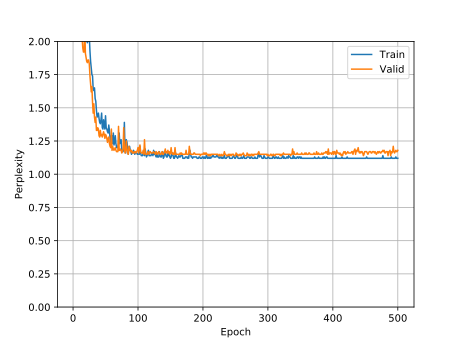
\includegraphics[width=\textwidth]{../results/monument2_1/run1/transformer_iwslt_de_en/ppls.png}
\caption{Transformer}
\label{fig:monu1 transformer ppl}
\end{subfigure}
\hfill
\caption{Plots of perplexity on the training and validation set of Monument80 for each model}
\label{fig:monu1 ppls}
\end{figure}

Figure \ref{fig:monu1 ppls} shows the perplexity graphs on the Monument80 dataset. For this dataset, around 100 steps in the nmt are equivalent to an epoch in the fairseq. The trend of each model is similar with the MonumentNSpM dataset. Given the fact that this dataset contains more valid examples and less training examples than the MonumentNSpM dataset, the valid perplexities are mostly higher but still within the range 1 to 1.5. Slight overfittings are continued to be observed in Figure \ref{fig:monu1 nsm-bah ppl}, \ref{fig:monu1 nsm-luo ppl}, \ref{fig:monu1 gnmt4 ppl}, and \ref{fig:monu1 gnmt8 ppl}.

% Monument50 ppls
\begin{figure}[h]
\centering
\begin{subfigure}{0.3\textwidth}
\includegraphics[width=\textwidth]{../results/monument2_2/run1/neural_sparql_machine/ppls.png} 
\caption{NSpM}
\label{fig:monu2 nsm ppl}
\end{subfigure}
\hfill
\begin{subfigure}{0.3\textwidth}
\includegraphics[width=\textwidth]{../results/monument2_2/run1/neural_sparql_machine_bahdanau_attention/ppls.png}
\caption{NSpM+Att1}
\label{fig:monu2 nsm-bah ppl}
\end{subfigure}
\hfill
\begin{subfigure}{0.3\textwidth}
\includegraphics[width=\textwidth]{../results/monument2_2/run1/neural_sparql_machine_luong_attention/ppls.png} 
\caption{NSpM+Att2}
\label{fig:monu2 nsm-luo ppl}
\end{subfigure}
\hfill
\begin{subfigure}{0.3\textwidth}
\includegraphics[width=\textwidth]{../results/monument2_2/run1/lstm_luong_wmt_en_de/ppls.png}
\caption{LSTM\_Luong}
\label{fig:monu2 lstm ppl}
\end{subfigure}
\hfill
\begin{subfigure}{0.3\textwidth}
\includegraphics[width=\textwidth]{../results/monument2_2/run1/wmt16_gnmt_4_layer/ppls.png} 
\caption{GNMT-4}
\label{fig:monu2 gnmt4 ppl}
\end{subfigure}
\hfill
\begin{subfigure}{0.3\textwidth}
\includegraphics[width=\textwidth]{../results/monument2_2/run1/wmt16_gnmt_8_layer/ppls.png}
\caption{GNMT-8}
\label{fig:monu2 gnmt8 ppl}
\end{subfigure}
\hfill
\begin{subfigure}{0.3\textwidth}
\includegraphics[width=\textwidth]{../results/monument2_2/run2/fconv_wmt_en_de/ppls.png} 
\caption{ConvS2S}
\label{fig:monu2 convs2s ppl}
\end{subfigure}
\hfill
\begin{subfigure}{0.3\textwidth}
\includegraphics[width=\textwidth]{../results/monument2_2/run1/transformer_iwslt_de_en/ppls.png}
\caption{Transformer}
\label{fig:monu2 transformer ppl}
\end{subfigure}
\hfill
\caption{Plots of perplexity on the training and validation set of Monument50 for each model}
\label{fig:monu2 ppls}
\end{figure}

Next, in order to assess the complexity of the monument dataset, we experimented on the Monument50 by further reducing the number of training examples but keeping the same size of the valid set. Here, one epoch is equivalent to 60 steps. The perplexity graphs are shown in Figure \ref{fig:monu2 ppls}. Although the training size is nearly half cut, it appears that the performance on the valid set are not much affected, especially for LSTM\_Luong, ConvS2S, and Transformer which are all implemented in the fairseq. This phenomenon is also reflected on BLEU scores in Table \ref{table:monu50 bleu} and Table \ref{table:monu80 bleu}.  

% LC-QUAD ppls
\begin{figure}[h]
\centering
\begin{subfigure}{0.3\textwidth}
\includegraphics[width=\textwidth]{../results/lc-quad1/run1/neural_sparql_machine/ppls.png} 
\caption{NSpM}
\label{fig:lcquad nsm ppl}
\end{subfigure}
\hfill
\begin{subfigure}{0.3\textwidth}
\includegraphics[width=\textwidth]{../results/lc-quad1/run1/neural_sparql_machine_bahdanau_attention/ppls.png}
\caption{NSpM+Att1}
\label{fig:lcquad nsm-bah ppl}
\end{subfigure}
\hfill
\begin{subfigure}{0.3\textwidth}
\includegraphics[width=\textwidth]{../results/lc-quad1/run1/neural_sparql_machine_luong_attention/ppls.png} 
\caption{NSpM+Att2}
\label{fig:lcquad nsm-luo ppl}
\end{subfigure}
\hfill
\begin{subfigure}{0.3\textwidth}
\includegraphics[width=\textwidth]{../results/lc-quad1/run1/lstm_luong_wmt_en_de/ppls.png}
\caption{LSTM\_Luong}
\label{fig:lcquad lstm ppl}
\end{subfigure}
\hfill
\begin{subfigure}{0.3\textwidth}
\includegraphics[width=\textwidth]{../results/lc-quad1/run1/wmt16_gnmt_4_layer/ppls.png} 
\caption{GNMT-4}
\label{fig:lcquad gnmt4 ppl}
\end{subfigure}
\hfill
\begin{subfigure}{0.3\textwidth}
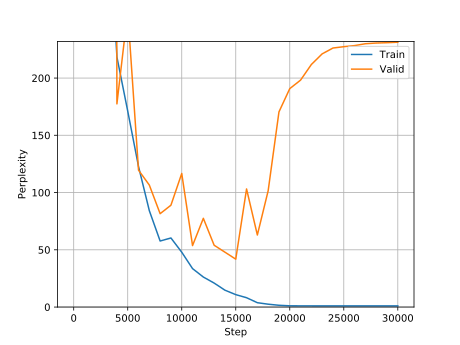
\includegraphics[width=\textwidth]{../results/lc-quad1/run1/wmt16_gnmt_8_layer/ppls.png}
\caption{GNMT-8}
\label{fig:lcquad gnmt8 ppl}
\end{subfigure}
\hfill
\begin{subfigure}{0.3\textwidth}
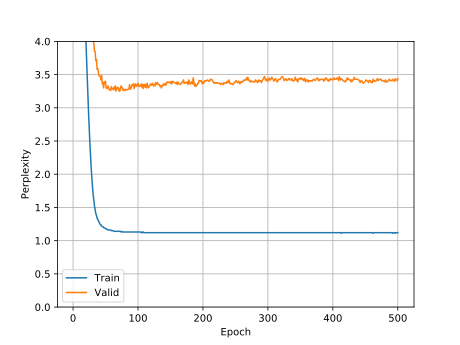
\includegraphics[width=\textwidth]{../results/lc-quad1/run2/fconv_wmt_en_de/ppls.png} 
\caption{ConvS2S}
\label{fig:lcquad convs2s ppl}
\end{subfigure}
\hfill
\begin{subfigure}{0.3\textwidth}
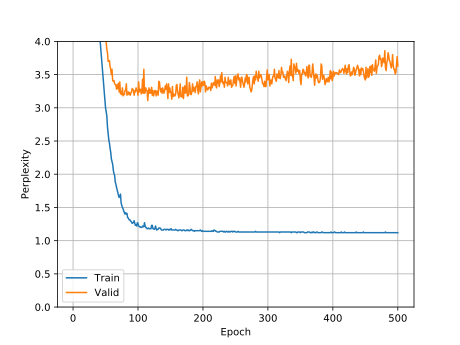
\includegraphics[width=\textwidth]{../results/lc-quad1/run1/transformer_iwslt_de_en/ppls.png}
\caption{Transformer}
\label{fig:lcquad transformer ppl}
\end{subfigure}
\hfill
\caption{Plots of perplexity on the training and validation set of LC-QUAD for each model}
\label{fig:lcquad ppls}
\end{figure}

In the perplexity graphs on the LC-QUAD dataset shown in Figure \ref{fig:lcquad ppls}, we observed a noticeable difference between five models (Figure \ref{fig:lcquad nsm ppl}, \ref{fig:lcquad nsm-bah ppl}, \ref{fig:lcquad nsm-luo ppl}, \ref{fig:lcquad gnmt4 ppl} and \ref{fig:lcquad gnmt8 ppl} have shown serious overfitting at the time of convergence) implemented by the nmt and three models (Figure \ref{fig:lcquad lstm ppl}, \ref{fig:lcquad convs2s ppl} and \ref{fig:lcquad transformer ppl}) implemented by the fairseq. LC-QUAD is much smaller but more complicated compared to other datasets. It only takes 34 steps to finish training an epoch inside the nmt framework. Most of the models have difficulty of providing low perplexity on the valid set, among which GNMT-8 performed the worst and ConvS2S the best. 

%DBNQA ppls
\begin{figure}[h]
\centering
\begin{subfigure}{0.3\textwidth}
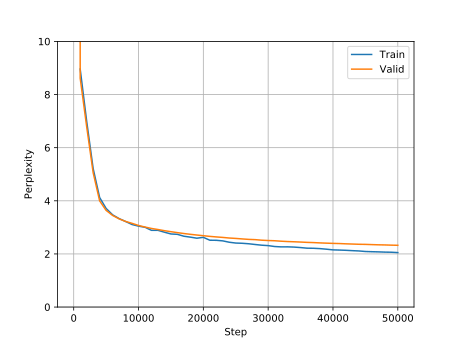
\includegraphics[width=\textwidth]{../results/dbnqa1/run1/neural_sparql_machine/ppls.png} 
\caption{NSpM}
\label{fig:dbnqa nsm ppl}
\end{subfigure}
\hfill
\begin{subfigure}{0.3\textwidth}
\includegraphics[width=\textwidth]{../results/dbnqa1/run1/neural_sparql_machine_bahdanau_attention/ppls.png}
\caption{NSpM+Att1}
\label{fig:dbnqa nsm-bah ppl}
\end{subfigure}
\hfill
\begin{subfigure}{0.3\textwidth}
\includegraphics[width=\textwidth]{../results/dbnqa1/run1/neural_sparql_machine_luong_attention/ppls.png} 
\caption{NSpM+Att2}
\label{fig:dbnqa nsm-luo ppl}
\end{subfigure}
\hfill
\begin{subfigure}{0.3\textwidth}
\includegraphics[width=\textwidth]{../results/dbnqa1/run1/lstm_luong_wmt_en_de/ppls.png}
\caption{LSTM\_Luong}
\label{fig:dbnqa lstm ppl}
\end{subfigure}
\hfill
\begin{subfigure}{0.3\textwidth}
\includegraphics[width=\textwidth]{../results/dbnqa1/run1/wmt16_gnmt_4_layer/ppls.png} 
\caption{GNMT-4}
\label{fig:dbnqa gnmt4 ppl}
\end{subfigure}
\hfill
\begin{subfigure}{0.3\textwidth}
\includegraphics[width=\textwidth]{../results/dbnqa1/run1/wmt16_gnmt_8_layer/ppls.png}
\caption{GNMT-8}
\label{fig:dbnqa gnmt8 ppl}
\end{subfigure}
\hfill
\begin{subfigure}{0.3\textwidth}
\includegraphics[width=\textwidth]{../results/dbnqa1/run1/fconv_wmt_en_de/ppls.png} 
\caption{ConvS2S}
\label{fig:dbnqa convs2s ppl}
\end{subfigure}
\hfill
\begin{subfigure}{0.3\textwidth}
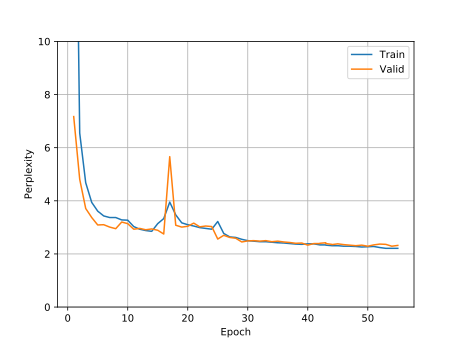
\includegraphics[width=\textwidth]{../results/dbnqa1/run1/transformer_iwslt_de_en/ppls.png}
\caption{Transformer}
\label{fig:dbnqa transformer ppl}
\end{subfigure}
\hfill
\caption{Plots of perplexity on the training and validation set of DBNQA for each model}
\label{fig:dbnqa ppls}
\end{figure}

Finally, Figure \ref{fig:dbnqa ppls} demonstrates the perplexities on the DBNQA dataset. Across all of the models, no evident overfitting is spotted. In a batch size of 128, an epoch of DBNQA takes nearly 5600 training steps. Due to the large size of DBNQA, some models like NSpM and GNMT-8 have shown rather slow or incomplete convergence since the maximum training steps for them (50k and 30k) are just equivalent to a small number (10 and 6) of epochs. Despite that, all of the models have reached a perplexity of at least 2 on the valid set, where NSpM+Att1, NSpM+Att2, and ConvS2S have achieved lower than 2 as shown in Figure \ref{fig:dbnqa nsm-bah ppl}, \ref{fig:dbnqa nsm-luo ppl}, and \ref{fig:dbnqa convs2s ppl}.

\subsection{BLEU Scores}

The BLEU scores of the best checkpoint from each model are stated in Table \ref{table:monu600 bleu}-\ref{table:dbnqa bleu}. In each table, we primarily listed the BLEU scores on the valid and test set as well as the corresponding index of step or epoch of the selected model checkpoint. In order to refer to the state of the checkpoint at that step or epoch, we also reported the perplexities measured on the training and validation set.

\begin{table}[h]
\centering
\caption{BLEU scores and other information of the best checkpoint from each model on MonumentNSpM dataset}
\label{table:monu600 bleu}
\begin{tabular}{c|c|c|c|c|c}
Models & Train ppl & Valid ppl & \textbf{Valid BLEU} & \textbf{Test BLEU} & Step / Epoch \\
\hline
NSpM & 1.00 & 1.09 & 80.43 & 80.28 & Step 29k \\
NSpM+Att1 & 1.01 & 1.16 & 80.36 & 80.58 & Step 14k \\
NSpM+Att2 & 1.01 & 1.14 & 80.88 & 80.03 & Step 9k \\
GNMT-4 & 1.03 & 1.11 & 80.12 & 79.53 & Step 11k \\
GNMT-8 & 1.04 & 1.15 & 79.30 & 79.07 & Step 10k \\
LSTM\_Luong & 1.11 & 1.19 & 92.39 & 91.67 & Epoch 500 \\
ConvS2S & 1.11 & 1.14 & \textbf{98.35} & \textbf{97.12} & Epoch 500 \\
Transformer & 1.13 & 1.09 & 95.25 & 95.31 & Epoch 138 \\
\end{tabular}
\end{table}

In Table \ref{table:monu600 bleu}-\ref{table:monu50 bleu}, we reported the BLEU scores on three splits of the monument dataset. In all of these experiments, ConvS2S performed the best. It is also the case that LSTM\_Luong, ConvS2S, and Transformer outperformed other models by a large margin (about 10-15 BLEUs), most evident on the MonumentNSpM experiments.

\begin{table}[h]
\centering
\caption{BLEU scores and other information of the best checkpoint from each model on Monument80 dataset}
\label{table:monu80 bleu}
\begin{tabular}{c|c|c|c|c|c}
Models & Train ppl & Valid ppl & \textbf{Valid BLEU} & \textbf{Test BLEU} & Step / Epoch \\
\hline
NSpM & 1.00 & 1.21 & 87.55 & 87.03 & Step 44k \\
NSpM+Att1 & 1.00 & 1.44 & 87.82 & 87.34 & Step 44k \\
NSpM+Att2 & 1.00 & 1.44 & 87.99 & 87.37 & Step 34k \\
GNMT-4 & 1.00 & 1.31 & 85.94 & 85.39 & Step 30k \\
GNMT-8 & 1.01 & 1.32 & 84.94 & 84.14 & Step 30k \\
LSTM\_Luong & 1.11 & 1.24 & 96.35 & 96.12 & Epoch 200 \\
ConvS2S & 1.11 & 1.19 & \textbf{96.74} & \textbf{96.47} & Epoch 500 \\
Transformer & 1.12 & 1.14 & 95.16 & 94.87 & Epoch 267 \\
\end{tabular}
\end{table}

\begin{table}[h]
\centering
\caption{BLEU scores and other information of the best checkpoint from each model on Monument50 dataset}
\label{table:monu50 bleu}
\begin{tabular}{c|c|c|c|c|c}
Models & Train ppl & Valid ppl & \textbf{Valid BLEU} & \textbf{Test BLEU} & Step / Epoch \\
\hline
NSpM & 1.00 & 1.29 & 85.19 & 85.54 & Step 50k \\
NSpM+Att1 & 1.00 & 1.60 & 85.98 & 86.17 & Step 50k \\
NSpM+Att2 & 1.00 & 1.62 & 86.60 & 86.52 & Step 50k \\
GNMT-4 & 1.00 & 1.41 & 82.92 & 83.01 & Step 30k \\
GNMT-8 & 1.00 & 1.59 & 80.35 & 80.76 & Step 30k \\
LSTM\_Luong & 1.11 & 1.26 & 94.05 & 94.75 & Epoch 500 \\
ConvS2S & 1.11 & 1.20 & \textbf{96.44} & \textbf{96.62} & Epoch 500 \\
Transformer & 1.14 & 1.17 & 93.80 & 93.92 & Epoch 108 \\
\end{tabular}
\end{table}

\begin{table}[h]
\centering
\caption{BLEU scores and other information of the best checkpoint from each model on LC-QUAD dataset}
\label{table:lc-quad bleu}
\begin{tabular}{c|c|c|c|c|c}
Models & Train ppl & Valid ppl & \textbf{Valid BLEU} & \textbf{Test BLEU} & Step / Epoch \\
\hline
NSpM & 1.00 & 16.46 & 43.91 & 43.50 & Step 20k \\
NSpM+Att1 & 1.00 & 56.23 & 52.68 & 50.13 & Step 40k \\
NSpM+Att2 & 1.00 & 43.20 & 53.03 & 50.86 & Step 41k \\
GNMT-4 & 1.00 & 33.76 & 43.69 & 42.71 & Step 9k \\
GNMT-8 & 1.01 & 229.96 & 44.32 & 43.91 & Step 27k \\
LSTM\_Luong & 1.12 & 4.92 & 52.43 & 51.06 & Epoch 218 \\
ConvS2S & 1.14 & 3.25 & \textbf{61.89} & \textbf{59.54} & Epoch 71 \\
Transformer & 1.16 & 3.15 & 58.99 & 57.43 & Epoch 163 \\
\end{tabular}
\end{table}

Table \ref{table:lc-quad bleu} shows the performance of each model on the LC-QUAD dataset. The models all achieved relatively lower BLEU scores on this dataset as well as higher perplexities compared to other datasets. Another thing to notice is that the best checkpoints selected here are all from the middle stages of the training, which correlates with the potential overfittings exhibited in Figure \ref{fig:lcquad ppls}.

Table \ref{table:dbnqa bleu} displays the BLEU results on the DBNQA dataset. The ConvS2S model outperformed the NSpM model by around 30 BLEU points here, which is the largest model performance difference across all the datasets. It is also worth mentioning that the scores of the Transformer model declined to the third worst and the results of the NSpM with attentions raised to the second best in this dataset, which is usually the opposite in other datasets.

\begin{table}[h]
\centering
\caption{BLEU scores and other information of the best checkpoint from each model on DBNQA dataset}
\label{table:dbnqa bleu}
\begin{tabular}{c|c|c|c|c|c}
Models & Train ppl & Valid ppl & \textbf{Valid BLEU} & \textbf{Test BLEU} & Step / Epoch \\
\hline
NSpM & 2.05 & 2.32 & 65.89 & 65.92 & Step 50k \\
NSpM+Att1 & 1.07 & 1.42 & 89.87 & 89.87 & Step 50k \\
NSpM+Att2 & 1.05 & 1.37 & 91.51 & 91.50 & Step 50k \\
GNMT-4 & 1.74 & 2.24 & 69.65 & 69.61 & Step 30k \\
GNMT-8 & 2.13 & 2.43 & 68.43 & 68.41 & Step 30k \\
LSTM\_Luong & 1.90 & 2.15 & 77.64 & 77.67 & Epoch 55 \\
ConvS2S & 1.12 & 1.25 & \textbf{96.05} & \textbf{96.07} & Epoch 54 \\
Transformer & 2.21 & 3.34 & 68.68 & 68.82 & Epoch 53 \\
\end{tabular}
\end{table}

\section{Discussion} \label{section:discussion}










\chapter{Conclusion} \label{chapter:conclusion}


\section{Summary} \label{section:summary}

The Semantic Web is gradually changing the way the information and data are stored on the Web. It enables a new form of accessing the knowledge located in various places - through Linked Data. However, most of the linked datasets, such as DBpedia, has not yet unleashed their great potentials because of the specialized query languages like SPARQL that are necessary to be mastered for accessing this data and the huge gap between it and the natural languages used by the humans. We believe this gap could be bridged by the application of Neural Machine Translation models on the specific task of translating natural language to SPARQL. 

In this thesis, after thorough investigation on various related datasets and NMT architectures, three representative categories of models in NMT were selected to be tested on three English-SPARQL datasets. We carried out 40 experiments which consist of training 8 models with different configurations in architecture and parameters on 5 experimental datasets after splitting and preprocessing three originally examined ones. We demonstrated the results in perplexity graphs and BLEU score tables and discussed their implications.

It has been found that the ConvS2S model consistently outperformed other models in all of the experiments in terms of convergence and translation quality, and the DBNQA dataset is so far the most appropriate English-SPARQL dataset for the training and testing of NMT models. Based on the results, we also discussed the relationship between the perplexity and BLEU and compared the difference between our specific task and the common task in the field of NMT. Finally, three primary limitations of our experiments were pointed out, which mostly impacted the results in the aspects of training and evaluation.

\section{Outlook} \label{section:outlook}

Although the experiments have shown encouraging results in this thesis, there is some future work that deserves to be attached importance to specifically for the task of translating natural language to SPARQL. The first is to establish a NL-SPARQL dataset that suits the requirements of training deep neural networks while preserving the complexity of the question and query types. This could be potentially fulfilled by taking the templates from the DBNQA and deploying the generation methods of LC-QUAD, as stated in Section \ref{section:datasets}. The second is designing a unique metric to replace BLEU for better evaluating the quality of the translated queries, which should not only focus on the sentence structures but also on the semantics and execution results in practical situations. Last but not least, with the realization of aforementioned outlooks and acknowledgements of certain limitations specified in Section \ref{subsection:limitation}, it is well worth training these or even more NMT models on this task in a more standardized way. 







\end{document}
